% !TEX root = ../../../main.tex
% 第二部分第四章第二节：第二类曲线积分与曲面积分
\section{第二类曲线积分与曲面积分}
\subsection*{第二类曲线积分}
设空间力场为
\[
\boldsymbol F(x,y,z)=P(x,y,z)\boldsymbol i+Q(x,y,z)\boldsymbol j+R(x,y,z)\boldsymbol k.
\]
物体沿有向曲线 $L$ 从 $A$ 运动到 $B$，力场所做的功可由下面的积分表示。
\begin{definition}
设 $L$ 为有向光滑曲线，$\boldsymbol F$ 在 $L$ 上有界。沿指定方向取分点 $A=P_0,P_1,\ldots,P_n=B$。记小弧段 $\wideparen{P_{k-1}P_k}$ 的长度为 $\Delta s_k$，在其上任取一点 $X_k=(\xi_k,\eta_k,\zeta_k)$，以 $\boldsymbol\tau(X_k)$ 表示该点沿曲线指定方向的单位切向量。小弧段上的功近似为
\[
\Delta W_k\approx\boldsymbol F(X_k)\cdot\boldsymbol\tau(X_k)\Delta s_k.
\]
作和式
\[
S_n=\sum_{k=1}^n\boldsymbol F(X_k)\cdot\boldsymbol\tau(X_k)\Delta s_k,
\qquad \lambda=\max_k\Delta s_k.
\]
若 $\lambda\to0$ 时该和式有有限极限，且与划分及取点无关，则称其为 $\boldsymbol F$ 沿 $L$ 的第二类曲线积分，记为
\[
I=\int_L\boldsymbol F\cdot\boldsymbol\tau\,\dd s
=\lim_{\lambda\to0}S_n.
\]
记 $\dd\boldsymbol s=\boldsymbol\tau\,\dd s$，也写作 $\displaystyle\int_L\boldsymbol F\cdot\dd\boldsymbol s$。
\end{definition}
若单位切向量与三个坐标轴的夹角为 $\alpha,\beta,\gamma$，则
\[
\boldsymbol\tau=\cos\alpha\,\boldsymbol i+\cos\beta\,\boldsymbol j+\cos\gamma\,\boldsymbol k,
\]
从而第二类曲线积分化为第一类曲线积分：
\[
I=\int_L(P\cos\alpha+Q\cos\beta+R\cos\gamma)\,\dd s.
\]
沿曲线有 $\dd x=\cos\alpha\,\dd s$、$\dd y=\cos\beta\,\dd s$、$\dd z=\cos\gamma\,\dd s$，因此又记为
\[
I=\int_LP\,\dd x+Q\,\dd y+R\,\dd z.
\]
特别地，若 $L$ 是 $xy$ 平面上的有向光滑曲线，则
\begin{align*}
\int_LP\,\dd x+Q\,\dd y
&=\int_L(P\cos\alpha+Q\cos\beta)\,\dd s\\
&=\int_L(P\cos\alpha+Q\sin\alpha)\,\dd s.
\end{align*}
这里平面情形的 $\alpha$ 是有向切向量与 $x$ 轴正向所成的有向角。

\begin{proposition}
\begin{enumerate}
\item 方向性：记 $-L$ 为 $L$ 的反向曲线，则
\[
\int_{-L}\boldsymbol F\cdot\boldsymbol\tau\,\dd s
=-\int_L\boldsymbol F\cdot\boldsymbol\tau\,\dd s.
\]
\item 线性性：若 $\boldsymbol F,\boldsymbol G$ 沿 $L$ 可积，$a,b$ 为常数，则
\[
\int_L(a\boldsymbol F+b\boldsymbol G)\cdot\boldsymbol\tau\,\dd s
=a\int_L\boldsymbol F\cdot\boldsymbol\tau\,\dd s+b\int_L\boldsymbol G\cdot\boldsymbol\tau\,\dd s.
\]
\item 路径可加性：若有向曲线 $L=L_1+L_2$ 由方向相容的两段拼成，则沿 $L$ 可积当且仅当沿两段均可积，且
\[
\int_L\boldsymbol F\cdot\boldsymbol\tau\,\dd s
=\int_{L_1}\boldsymbol F\cdot\boldsymbol\tau\,\dd s+\int_{L_2}\boldsymbol F\cdot\boldsymbol\tau\,\dd s.
\]
\end{enumerate}
\end{proposition}
% 原图未展开这三条性质的证明。
\begin{proof}
\begin{enumerate}
\item 反向后单位切向量变为 $-\boldsymbol\tau$，弧长微元不变，故每个对应积分和变号，取极限即得结论。
\item 每个积分和关于被积向量场都是线性的，将和式拆开并分别取极限，便得到所述等式。
\item 在拼接点处分开划分，积分和即分成两段上的积分和。反之，把标量函数 $\boldsymbol F\cdot\boldsymbol\tau$ 看作第一类曲线积分的被积函数，利用其路径可加性及可积性的限制性质，得到可积性的等价关系与等式。分段光滑曲线的有限个拼接点不影响积分值。
\end{enumerate}
\end{proof}

\begin{theorem}
设 $L$ 的光滑参数表示为
\[
x=x(t),\quad y=y(t),\quad z=z(t),\qquad a\le t\le b,
\]
参数从 $a$ 增至 $b$ 时与 $L$ 的方向一致，且 $P,Q,R$ 在 $L$ 上连续，则
\begin{align*}
\int_LP\,\dd x+Q\,\dd y+R\,\dd z
=\int_a^b\bigl[&P(x(t),y(t),z(t))x'(t)\\
&+Q(x(t),y(t),z(t))y'(t)\\
&+R(x(t),y(t),z(t))z'(t)\bigr]\,\dd t.
\end{align*}
\end{theorem}
\begin{proof}
记 $\boldsymbol r(t)=(x(t),y(t),z(t))$ 及 $v(t)=\lVert\boldsymbol r'(t)\rVert>0$，则
\[
\boldsymbol\tau(\boldsymbol r(t))=\frac{\boldsymbol r'(t)}{v(t)},
\qquad \dd s=v(t)\,\dd t.
\]
对参数划分 $a=t_0<\cdots<t_n=b$，在对应弧段上取点 $\boldsymbol r(\bar t_k)$。由积分中值定理，可取 $\theta_k\in[t_{k-1},t_k]$ 使
\[
\Delta s_k=v(\theta_k)\Delta t_k.
\]
因此
\[
S_n=\sum_{k=1}^n
\boldsymbol F(\boldsymbol r(\bar t_k))\cdot
\frac{\boldsymbol r'(\bar t_k)}{v(\bar t_k)}
v(\theta_k)\Delta t_k.
\]
由于 $v$ 连续且在闭区间上有正的下界，弧长划分模长趋于零时，参数划分模长也趋于零；由一致连续性，$v(\theta_k)/v(\bar t_k)\to1$ 一致成立。于是上式与
\[
\sum_{k=1}^n\boldsymbol F(\boldsymbol r(\bar t_k))\cdot\boldsymbol r'(\bar t_k)\Delta t_k
\]
之差趋于零。后者是连续函数 $\boldsymbol F(\boldsymbol r(t))\cdot\boldsymbol r'(t)$ 的 Riemann 和，其极限即为所述积分。
\end{proof}

特别地，若空间曲线以 $x$ 为参数，方程为 $y=y(x),z=z(x)$，方向为 $x:a\to b$，则
\[
\begin{aligned}
\int_LP\,\dd x+Q\,\dd y+R\,\dd z
=\int_a^b\bigl[&P(x,y(x),z(x))\\
&+Q(x,y(x),z(x))y'(x)\\
&+R(x,y(x),z(x))z'(x)\bigr]\,\dd x.
\end{aligned}
\]
对于平面有向光滑曲线 $x=x(t),y=y(t)$，有
\[
\int_LP\,\dd x+Q\,\dd y
=\int_a^b[P(x(t),y(t))x'(t)+Q(x(t),y(t))y'(t)]\,\dd t.
\]
若平面曲线方程为 $y=y(x)$，方向为 $x:a\to b$，则
\[
\int_LP\,\dd x+Q\,\dd y
=\int_a^b[P(x,y(x))+Q(x,y(x))y'(x)]\,\dd x.
\]

\subsection*{曲面的侧}
\begin{definition}
设 $\Sigma$ 为光滑曲面，$P\in\Sigma$。从 $P$ 出发沿曲面上不经过边界的任一简单闭曲线连续移动一个单位法向量，回到 $P$ 时，若其方向总与出发时一致，则称 $\Sigma$ 为双侧曲面。
\end{definition}
在双侧曲面上选定一点的一个单位法向量，并连续地移动该法向量，就确定了曲面的一侧。两种相反的连续单位法向量场给出曲面的两侧，选定一侧的曲面称为定向曲面。

并非所有光滑曲面都是双侧曲面。例如，将长方形纸片 $ABCD$ 的一端扭转半周，使 $A$ 与 $C$、$B$ 与 $D$ 重合后粘接，得到 M\"obius 带。从一点出发沿带连续移动单位法向量，绕行一周回到原点时，法向量反向，因此它是单侧曲面。
\begin{center}
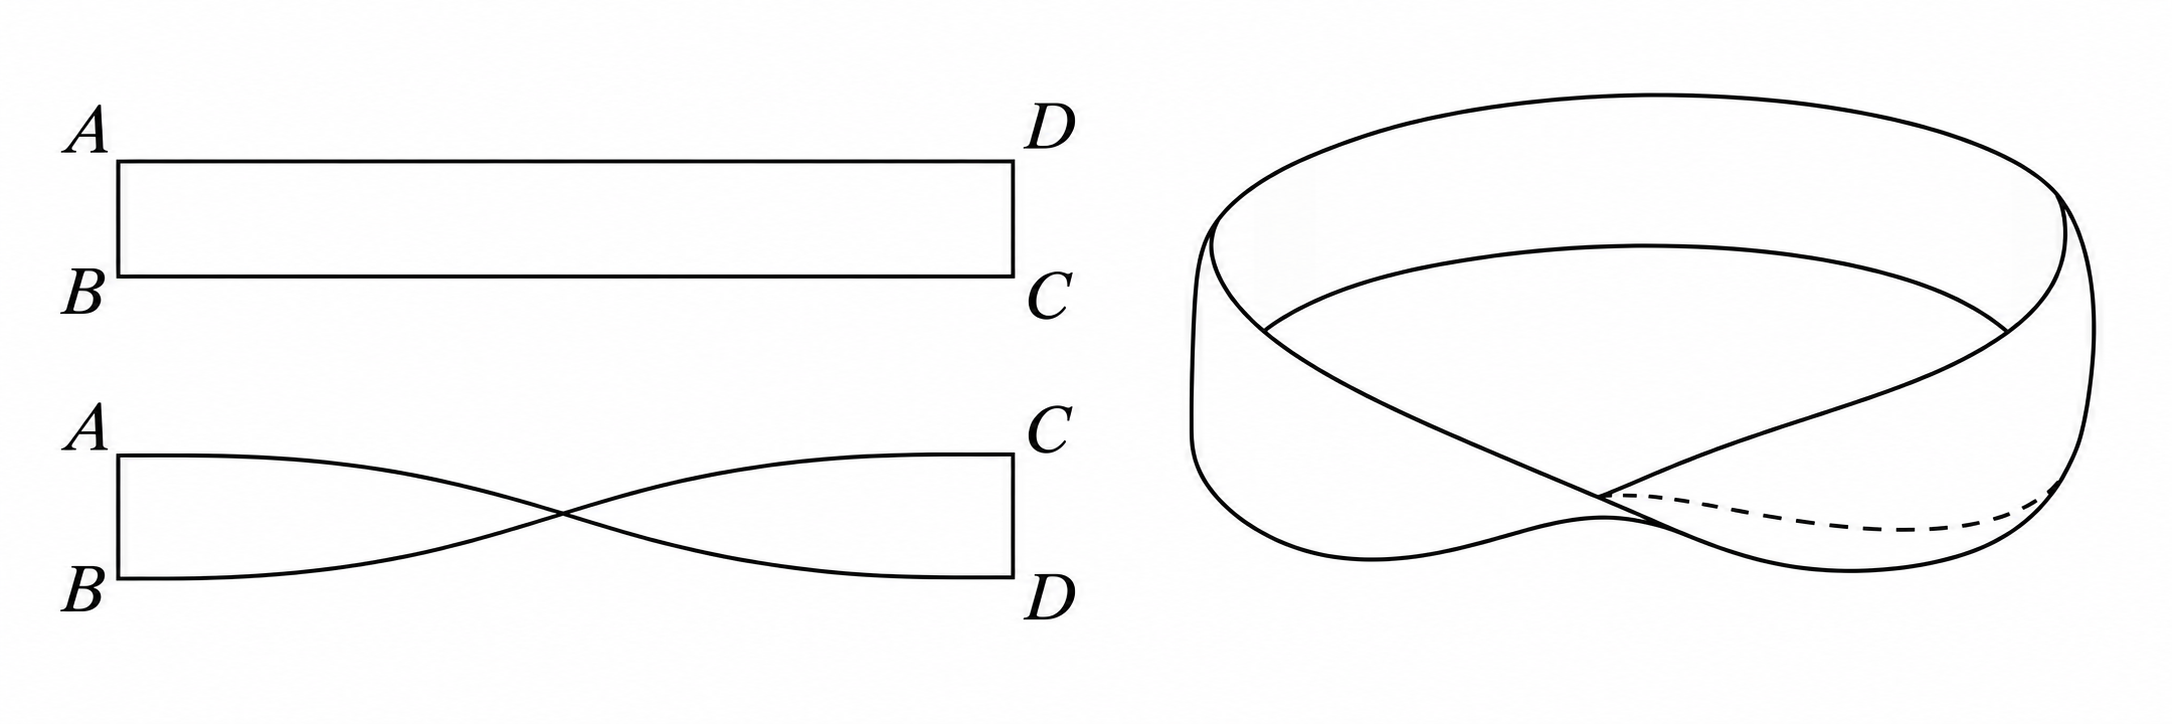
\includegraphics[width=0.92\linewidth]{figure/P2/mobius_redrawn_hd.png}
\end{center}
以下只讨论双侧曲面。注意，双侧曲面拼接后未必仍是双侧曲面；例如 M\"obius 带可以由两片双侧曲面拼接而成。

\subsection*{第二类曲面积分}
设曲面有参数表示
\[
x=x(u,v),\quad y=y(u,v),\quad z=z(u,v),\qquad (u,v)\in D,
\]
其中参数函数具有连续偏导数，记
\[
\boldsymbol r(u,v)=x(u,v)\boldsymbol i+y(u,v)\boldsymbol j+z(u,v)\boldsymbol k.
\]
在正则点，$\boldsymbol r_u\times\boldsymbol r_v\ne\boldsymbol0$。该向量同时垂直于两条参数曲线的切向量，给出曲面的一个法向方向。因而两种法向量可表示为
\[
\pm\boldsymbol r_u\times\boldsymbol r_v
=\pm\left(\frac{\partial(y,z)}{\partial(u,v)},
\frac{\partial(z,x)}{\partial(u,v)},
\frac{\partial(x,y)}{\partial(u,v)}\right).
\]
相应的单位法向量为
\[
\begin{aligned}
\boldsymbol n&=(\cos\alpha,\cos\beta,\cos\gamma)\\
&=\frac{\pm1}{\sqrt{EG-F^2}}
\left(\frac{\partial(y,z)}{\partial(u,v)},
\frac{\partial(z,x)}{\partial(u,v)},
\frac{\partial(x,y)}{\partial(u,v)}\right),
\end{aligned}
\]
其中
\[
EG-F^2=
\left(\frac{\partial(y,z)}{\partial(u,v)}\right)^2+
\left(\frac{\partial(z,x)}{\partial(u,v)}\right)^2+
\left(\frac{\partial(x,y)}{\partial(u,v)}\right)^2.
\]
对于这一正则参数表示，选定正负号便给出每一点的单位法向量。由于偏导数连续，所取单位法向量随点连续变化；在双侧曲面上使各参数片的法向选择相容，就确定了曲面的一侧。

% 以下按新提供图片的左栏、右栏顺序续写。
\subsection*{法向的选择}
以下以向上的一侧为例；对封闭曲面，则需按题意判断取外侧还是内侧。不能对整个球面都取向上的法向量，否则会在赤道处发生矛盾。例如，球面取外侧时，上半球的法向量指向上方，下半球的法向量指向下方。

对于由四个三角形面组成的四面体表面，也应分别判断各面的外侧，再使各面的取向与整体的外侧相容。
\begin{center}
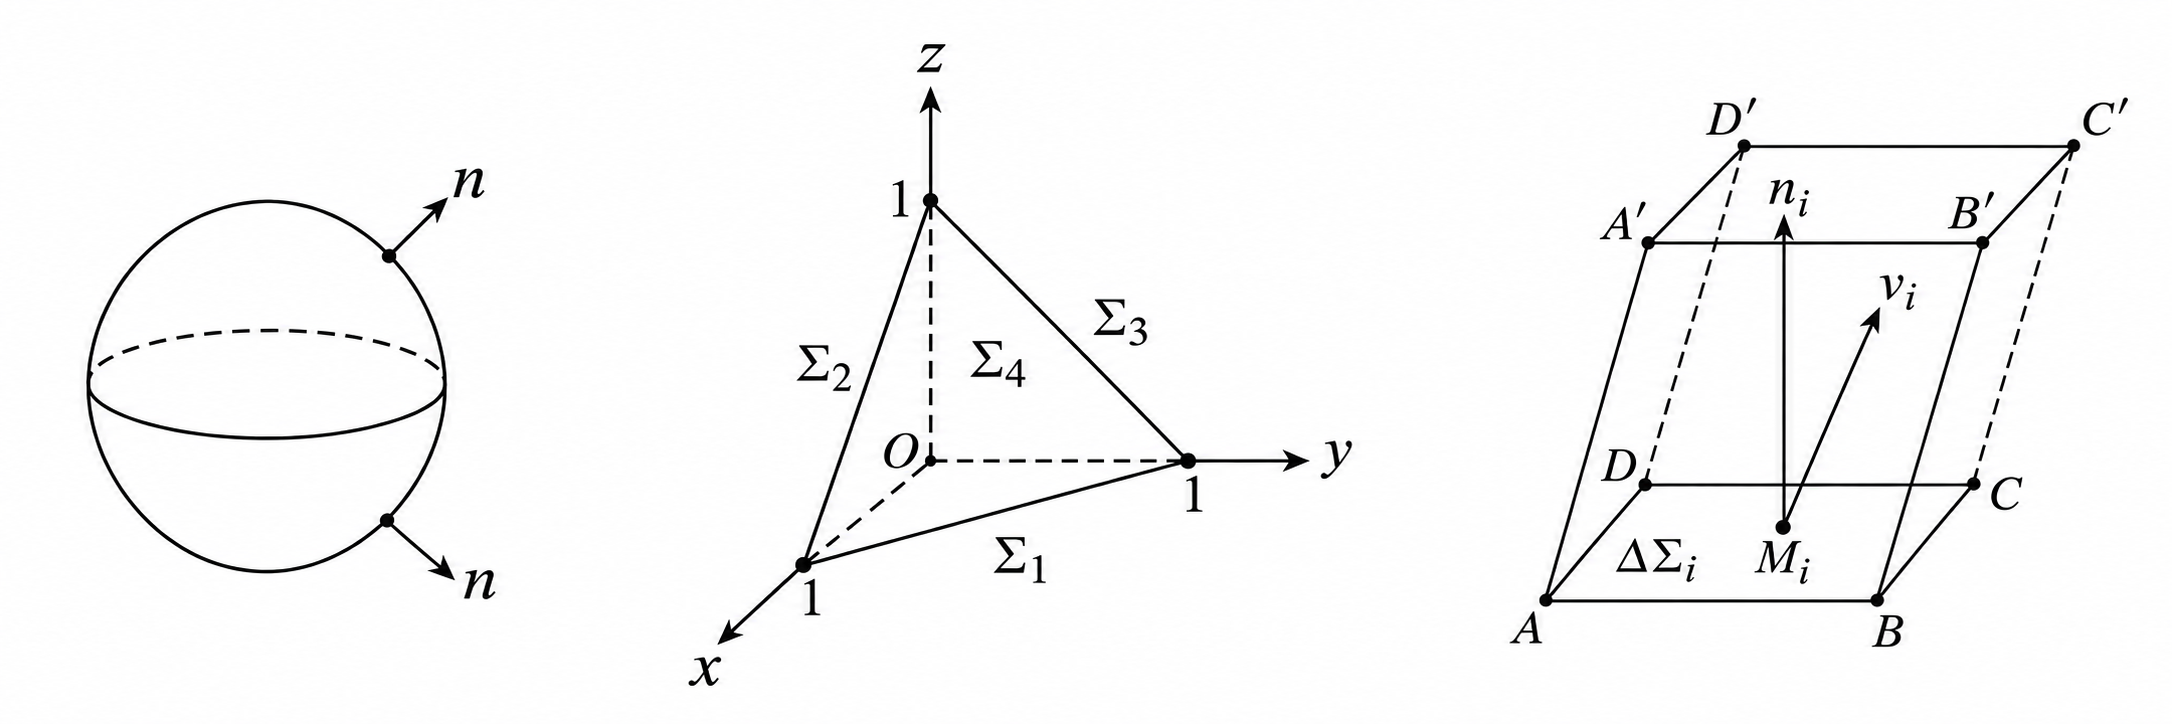
\includegraphics[width=0.98\linewidth]{figure/P2/flux_orientation_redrawn_hd.png}
\end{center}
若所取一侧的法向量的第三个分量为正，则比较
\[
(\boldsymbol r_u\times\boldsymbol r_v)_3
=\frac{\partial(x,y)}{\partial(u,v)}
=\begin{vmatrix}x_u&y_u\\x_v&y_v\end{vmatrix}.
\]
当这个行列式大于零时，取 $+\boldsymbol r_u\times\boldsymbol r_v$；小于零时，取 $-\boldsymbol r_u\times\boldsymbol r_v$。若该分量为零，就须通过其他非零分量判断，不能仅用第三个分量选定方向。

\subsection*{通量与第二类曲面积分的定义}
设有不可压缩流体，密度为 $1$，速度场为
\[
\boldsymbol v(x,y,z)=P(x,y,z)\boldsymbol i+Q(x,y,z)\boldsymbol j+R(x,y,z)\boldsymbol k.
\]
求单位时间内通过定向曲面 $\Sigma$ 的流量。用光滑曲线网将 $\Sigma$ 分成小曲面 $\Delta\Sigma_i$，其面积为 $\Delta S_i$。在每片上取点 $M_i=(\xi_i,\eta_i,\zeta_i)$，记该点的速度为 $\boldsymbol v_i$，所选一侧的单位法向量为
\[
\boldsymbol n_i=\cos\alpha_i\,\boldsymbol i+\cos\beta_i\,\boldsymbol j+\cos\gamma_i\,\boldsymbol k.
\]
在短时间 $\Delta t$ 内，流经小曲面片的体积近似为以该片为底、以 $\boldsymbol v_i\Delta t$ 为侧棱的斜柱体体积，其有向值为
\[
(\boldsymbol v_i\cdot\boldsymbol n_i)\Delta S_i\Delta t.
\]
除以 $\Delta t$，相加并令所有小片的最大直径 $\lambda$ 趋于零，得到单位时间内的总流量
\begin{align*}
\Phi
&=\lim_{\lambda\to0}\sum_i\boldsymbol v_i\cdot\boldsymbol n_i\Delta S_i\\
&=\displaystyle\iint_\Sigma(P\cos\alpha+Q\cos\beta+R\cos\gamma)\,\dd S.
\end{align*}
这里正值表示沿所选法向流出，负值表示反向流入。

\begin{definition}
设 $\Sigma$ 为定向光滑曲面，所选一侧的单位法向量为 $\boldsymbol n=(\cos\alpha,\cos\beta,\cos\gamma)$，向量场 $\boldsymbol F=(P,Q,R)$ 定义在 $\Sigma$ 上。称
\[
\displaystyle\iint_\Sigma\boldsymbol F\cdot\boldsymbol n\,\dd S
=\displaystyle\iint_\Sigma(P\cos\alpha+Q\cos\beta+R\cos\gamma)\,\dd S
\]
为 $\boldsymbol F$ 在 $\Sigma$ 上的第二类曲面积分，只要右端的第一类曲面积分存在。
\end{definition}
记 $\dd\boldsymbol S=\boldsymbol n\,\dd S$，也称为有向面积元，于是积分可记为 $\displaystyle\iint_\Sigma\boldsymbol F\cdot\dd\boldsymbol S$。并记
\[
\dd y\dd z=\cos\alpha\,\dd S,\qquad
\dd z\dd x=\cos\beta\,\dd S,\qquad
\dd x\dd y=\cos\gamma\,\dd S,
\]
则有
\[
\displaystyle\iint_\Sigma\boldsymbol F\cdot\boldsymbol n\,\dd S
=\displaystyle\iint_\Sigma P\,\dd y\wedge\dd z+Q\,\dd z\wedge\dd x+R\,\dd x\wedge\dd y.
\]
\[\dd y\wedge\dd z= \dd y\dd z,\quad   \dd z\wedge\dd x= \dd z\dd x,\quad  \dd x\wedge\dd y=\dd x\dd y\]
这里的 $\dd y\dd z,\dd z\dd x,\dd x\dd y$ 表示带方向的投影面积元，顺序与方向有关，不能当作普通的无向面积元任意交换次序。

\subsection*{计算公式}
对于正则参数表示 $\boldsymbol r(u,v)$，先按所选一侧确定符号 $\varepsilon\in\{1,-1\}$，使
\[
\boldsymbol n=\varepsilon\frac{\boldsymbol r_u\times\boldsymbol r_v}{\lVert\boldsymbol r_u\times\boldsymbol r_v\rVert}.
\]
由 $\dd S=\lVert\boldsymbol r_u\times\boldsymbol r_v\rVert\,\dd u\dd v$，得到
\begin{align*}
I&=\varepsilon\displaystyle\iint_D
\begin{vmatrix}P&Q&R\\x_u&y_u&z_u\\x_v&y_v&z_v\end{vmatrix}\,\dd u\dd v\\
&=\varepsilon\displaystyle\iint_D\left[
P\frac{\partial(y,z)}{\partial(u,v)}+
Q\frac{\partial(z,x)}{\partial(u,v)}+
R\frac{\partial(x,y)}{\partial(u,v)}\right]\,\dd u\dd v.
\end{align*}
其中 $P,Q,R$ 都在 $(x(u,v),y(u,v),z(u,v))$ 处取值。这同时给出了第二类曲面积分化为参数区域上二重积分的公式。

\begin{proposition}
\begin{enumerate}
\item 方向性：若 $-\Sigma$ 表示与 $\Sigma$ 取向相反的曲面，则
\[
\displaystyle\iint_{-\Sigma}\boldsymbol F\cdot\boldsymbol n\,\dd S
=-\displaystyle\iint_\Sigma\boldsymbol F\cdot\boldsymbol n\,\dd S.
\]
\item 线性性：若 $\boldsymbol F,\boldsymbol G$ 在 $\Sigma$ 上可积，$a,b$ 为常数，则
\[
\displaystyle\iint_\Sigma(a\boldsymbol F+b\boldsymbol G)\cdot\boldsymbol n\,\dd S
=a\displaystyle\iint_\Sigma\boldsymbol F\cdot\boldsymbol n\,\dd S
+b\displaystyle\iint_\Sigma\boldsymbol G\cdot\boldsymbol n\,\dd S.
\]
\item 曲面可加性：若 $\Sigma=\Sigma_1+\Sigma_2$，两片取向与整体一致且仅沿边界相接，则在 $\Sigma$ 上可积当且仅当在两片上均可积，并有
\[
\displaystyle\iint_\Sigma\boldsymbol F\cdot\boldsymbol n\,\dd S
=\displaystyle\iint_{\Sigma_1}\boldsymbol F\cdot\boldsymbol n\,\dd S
+\displaystyle\iint_{\Sigma_2}\boldsymbol F\cdot\boldsymbol n\,\dd S.
\]
\end{enumerate}
\end{proposition}
% 原图未展开三条性质的证明。
\begin{proof}
\begin{enumerate}
\item 取向反转使 $\boldsymbol n$ 变为 $-\boldsymbol n$，而无向面积元 $\dd S$ 不变，所以积分变号。
\item 将 $(a\boldsymbol F+b\boldsymbol G)\cdot\boldsymbol n$ 展开为 $a(\boldsymbol F\cdot\boldsymbol n)+b(\boldsymbol G\cdot\boldsymbol n)$，再用第一类曲面积分的线性性即得结论。
\item 将标量被积函数写为 $\boldsymbol F\cdot\boldsymbol n$，按两片曲面分别划分，积分和分成对应的两个和式。沿共同边界的光滑曲线面积为零，不影响积分；因此第一类曲面积分的可加性给出可积性的等价关系及所述等式。
\end{enumerate}
\end{proof}

\begin{example}
设 $\Sigma$ 是由坐标平面和 $x+y+z=1$ 围成的第一卦限内四面体的表面，取外侧，求
\[
I=\displaystyle\iint_\Sigma(x+1)\,\dd y\dd z+(y+1)\,\dd z\dd x+(z+1)\,\dd x\dd y.
\]
\end{example}
\begin{solution}
依次记 $z=0,y=0,x=0,x+y+z=1$ 上的四个面为 $\Sigma_1,\Sigma_2,\Sigma_3,\Sigma_4$，各取四面体外侧。记每个面上的积分为 $I_j$，则 $I=I_1+I_2+I_3+I_4$。

对于 $\Sigma_1$，取 $\boldsymbol r(x,y)=(x,y,0)$，参数域
\[
D_1=\{(x,y):x\ge0,\ y\ge0,\ x+y\le1\}.
\]
此时 $\boldsymbol r_x\times\boldsymbol r_y=(0,0,1)$，但外侧向下，须取负号。因此
\[
I_1=-\displaystyle\iint_{D_1}
\begin{vmatrix}x+1&y+1&1\\1&0&0\\0&1&0\end{vmatrix}\,\dd x\dd y
=-\displaystyle\iint_{D_1}1\,\dd x\dd y=-\frac12.
\]
对于 $\Sigma_2$，取 $\boldsymbol r(x,z)=(x,0,z)$，参数域 $D_2=\{(x,z):x,z\ge0,\ x+z\le1\}$。因为
\[
\boldsymbol r_x\times\boldsymbol r_z=(0,-1,0),
\]
它已经指向外侧，故取正号：
\[
I_2=\displaystyle\iint_{D_2}
\begin{vmatrix}x+1&1&z+1\\1&0&0\\0&0&1\end{vmatrix}\,\dd x\dd z
=-\displaystyle\iint_{D_2}1\,\dd x\dd z=-\frac12.
\]
同样，$\Sigma_3$ 的外法向量为 $(-1,0,0)$，其在 $yz$ 平面上的投影是面积为 $1/2$ 的三角形，且在此面上 $P=x+1=1$，从而
\[
I_3=-\frac12.
\]
对于 $\Sigma_4$，取
\[
\boldsymbol r(x,y)=(x,y,1-x-y),\qquad (x,y)\in D_1.
\]
有 $\boldsymbol r_x=(1,0,-1)$、$\boldsymbol r_y=(0,1,-1)$，故
\[
\boldsymbol r_x\times\boldsymbol r_y=(1,1,1).
\]
该向量指向外侧，取正号。于是
\begin{align*}
I_4&=\displaystyle\iint_{D_1}
\begin{vmatrix}x+1&y+1&2-x-y\\1&0&-1\\0&1&-1\end{vmatrix}\,\dd x\dd y\\
&=\displaystyle\iint_{D_1}4\,\dd x\dd y=2.
\end{align*}
因此
\[
I=-\frac12-\frac12-\frac12+2=\frac12.
\]
\end{solution}
